%Este trabalho está licenciado sob a Licença Creative Commons Atribuição-CompartilhaIgual 4.0 Internacional. Para ver uma cópia desta licença, visite https://creativecommons.org/licenses/by-sa/4.0/ ou envie uma carta para Creative Commons, PO Box 1866, Mountain View, CA 94042, USA.

\chapter{Função composta, injetora, sobrejetora e inversa}

\section{Função composta}

\begin{obs}
Consideremos duas funções $f: A \rightarrow B$ e $g: B \rightarrow C$, com $A, B \text{ e } C \subset \R$, tais que $Im(f) \subset B$. A função composta $g \circ f: A \rightarrow C$ é definida por:
\begin{equation*}
(g \circ f)(x)= g(f(x)). 
\end{equation*}

O seguinte diagrama ajuda a entender esta definição:

\begin{center}
    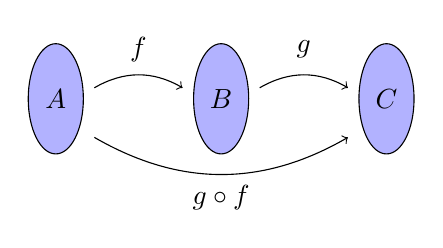
\begin{tikzpicture}[scale=0.7]
    \draw[fill=blue!30] (0,0) ellipse (0.5cm and 1cm);  
    \draw[fill=blue!30] (3,0) ellipse (0.5cm and 1cm);
    \draw[fill=blue!30] (6,0) ellipse (0.5cm and 1cm);
    \draw (0,0) node{$A$};
    \draw (3,0) node{$B$};
    \draw (6,0) node{$C$};
    \draw (1.5,0.9) node{$f$};
    \draw [->] (0.7,0.2) to [out=30,in=150] (2.3,0.2);
    \draw (4.5,0.9) node{$g$};
    \draw [->] (3.7,0.2) to [out=30,in=150] (5.3,0.2);
    \draw (3,-1.8) node{$g\circ f$};
    \draw [->] (0.7,-0.7) to [out=-30,in=-150] (5.3,-0.7);
    \end{tikzpicture}
\end{center}
\end{obs}


Em geral, $g\circ f \neq f\circ g$. Assim, devemos ter cuidado na ordem que é realizada composição.

Vejamos alguns exemplos de composições de funções $\R \to \R$.

\begin{exem}
Considerando a função linear $f(x)= -2x+4$, e a função quadrática $g(x)= x^2$. Chegamos as funções compostas 
\begin{enumerate}
\item [a)] $(f \circ g)(x)= f(g(x))= -2x^2 + 4$;
\item [b)] $(g \circ f)(x)= g(f(x))= (-2x+4)^2$.
\end{enumerate}
\end{exem}

\begin{exem}
Considere a função modular $f(x)= |x|$, e a função quadrática $g(x)= x^2-x-6$. Temos as seguintes funções compostas $\R \to \R$:
\begin{enumerate}
\item [a)] $(f \circ g)(x)= f(g(x))= |x^2-x-6|$;
\item [b)] $(g \circ f)(x)= g(f(x))= |x|^2 - |x|- 6$.
\end{enumerate}
\end{exem}

\begin{exem}
Com a função modular $f(x)= |x|$, e as funções lineares $g(x)= x+1$ e $h(x)= x-1$. Obtemos as seguintes funções compostas $\R \to \R$:
\begin{enumerate}
\item [a)] $(f \circ g)(x)= f(g(x)) \Rightarrow (f \circ g)(x)= |x+1|$;
\item [b)] $(f \circ h)(x)= f(h(x)) \Rightarrow (f \circ h)(x)= |x-1|$;
\item [c)] $(g \circ f)(x)= g(f(x)) \Rightarrow (g \circ f)(x)= |x|+1$;
\item [d)] $(h \circ f)(x)= h(f(x)) \Rightarrow (h \circ f)(x)= |x|-1$.
\end{enumerate}
Em cada um dos exemplos acima podemos observar a transformação do gráfico no plano cartesiano.
\end{exem}

O maior domínio de $g\circ f$ é o conjunto de todos os valores de $x$ no domínio de $f$ tais que $f(x)$ está no domínio de $g$. Em outras palavras, $(g\circ f)(x)$ está definida sempre que tanto $f(x)$ quanto $g(f(x))$ estiverem definidas.
Assim, 
\begin{equation*}
D(g \circ f)=\{ x\in D(f) \colon f(x) \in D(g)\}.    
\end{equation*}

\begin{exem}
    Dados $f(x)=\dfrac{x^2-4}{x-1}$ e $g(x)=\dfrac{1}{x}$ encontre o maior domínio de $g\circ f$.

    Temos de $D(f)=\R-\{1\}$ e $D(g)=\R-\{0\}$. Para $f(x)$ pertencer à $D(g)$, devemos ter que $f(x)\neq 0$, ou seja, $x\neq \pm 2$. Logo, o maior domínio de $g\circ f$ é
    \begin{equation*}
        D(g\circ f) = D(f)-{\pm 2} = \R-\{1,-4,4\}.
    \end{equation*}
\end{exem}

% \begin{exem}
% Considere as funções reais:
% \begin{eqnarray}
% f(x)= -x^2 + 8x -7
% \end{eqnarray}

% \begin{eqnarray}
% g(x)= \begin{cases}
%        g_1(x)= |x|, \text{ se } x \leqslant 9 \\
%        g_2(x)= x-3, \text{ se } x > 9
% 	  \end{cases}
% \end{eqnarray}
% Determine a função $(g \circ f)(x)= g(f(x))$.
% \begin{resol}
% Para fazer esta composição como a função $g$ é definida por partes precisamos qual é o conjunto imagem da função $f$. Note que $f$ é uma função do 2º grau com $a< 0$ logo concavidade voltada para baixo, o que nos diz que $Im(f)= (-\infty, y_v]$, por tanto basta calcular o $y_v$,
% \begin{eqnarray}
% y_v= \dfrac{- \Delta}{4a}= \dfrac{-(8^2-4.(-1).(-7))}{4.(-1)}= \dfrac{-36}{-4}= 9 \ .
% \end{eqnarray}
% Portanto, $Im(f)= (-\infty, 9]$. Assim, considerando a definição da função $g$, temos que
% \begin{eqnarray}
% (g \circ f)(x)= g(f(x))= g_1(f(x))= |-x^2 + 8x -7| \ .
% \end{eqnarray}
% \end{resol}
% \end{exem}

% \begin{exem}
% Considere as funções reais:
% \begin{eqnarray}
% f(x)= \begin{cases}
%       f_1(x)= -x^2+8x-7, \text{ se } x < 6 \\
%       f_2(x)= x-1, \text{ se } x \geqslant 6
%       \end{cases}
% \end{eqnarray}

% \begin{eqnarray}
% g(x)= \begin{cases}
%       g_1(x)= |x|, \text{ se } x < 5 \\
%       g_2(x)= 2x-5, \text{ se } 5 \leqslant x \leqslant 9 \\
%       g_3(x)= -x+22, \text{ se } x > 9
%       \end{cases}
% \end{eqnarray}
% Determine a função $(g \circ f)(x)= g(f(x))$.

%   \begin{figure}[H]
%  \centering
%     \fbox{\includegraphics[width=8cm]{./cap_funcao/figs/funcaoCompostaexem5}}
%     \caption{Gráfico da função $f$}
%   \end{figure}

% \begin{resol}
% Como a função $g$ está definida por partes, para fazer a composição precisamos entender o comportamento do conjunto imagem da função $f$. Observamos que:
% \begin{eqnarray}
% \begin{cases}
% f_1: (-\infty, 6) \to (-\infty, 9) \\
% f_2: [6, \infty) \to [5, \infty) \ .
% \end{cases}
% \end{eqnarray}
%  Com isso vemos que 
%  \begin{eqnarray}
% (g \circ f)(x)= \begin{cases}
%       g_1(f_1(x))= |-x^2+8x-7|, \text{ se } x < 2 \\
%       g_2(f_1(x))= 2*(-x^2+8x-7), \text{ se } 2 \leqslant x < 6 \\
%       g_2(f_2(x))= 2*(x-1)-5, \text{ se } 6 \leqslant x \leqslant 10 \\
%       g_3(f_2(x))= -(x-1)+22, \text{ se } x > 10
%       \end{cases}
% \end{eqnarray}
% \end{resol}
% \end{exem}

% \begin{exem}
% Considere as funções reais:
% \begin{eqnarray}
% f: [0, 2\pi] \to [-1, 1] \\
% f(x)= sen(x)
% \end{eqnarray}

% \begin{eqnarray}
% g(x)= \begin{cases}
%       g_1(x)= -2x, \text{ se } x < -1 \\
%       g_2(x)= 2|x|, \text{ se } -1 \leqslant x < 0 \\
%       g_3(x)= 4x, \text{ se } 0 \leqslant x \leqslant 1 \\
%       g_4(x)= x^2 + 3, \text{ se } x > 1
%       \end{cases}
% \end{eqnarray}
% Determine a função $(g \circ f)(x)= g(f(x))$.

% \begin{resol}
% Sabemos que $Im(f)= [-1, 1]$, logo
% \begin{eqnarray}
% g(f(x))= \begin{cases}
%       g_2(f(x))= 2|sen(x)|, \text{ se } \pi \leqslant x < 2\pi \\
%       g_3(f(x))= 4*sen(x), \text{ se }  0 \leqslant x \leqslant \pi \\
%       \end{cases}
% \end{eqnarray}
%   \begin{figure}[H]
%  \centering
%     \fbox{\includegraphics[width=8cm]{./cap_funcao/figs/funcaoCompostaexem6}}
%     \caption{Gráfico da função $(g \circ f)(x)$}
%   \end{figure}
% \end{resol}
% \end{exem}

% \begin{exem}
% As funções:
% \begin{itemize}
% \item $h_1: \R \setminus \{k*\pi \mid k \in \Z\} \to \R$ dada por $h_1(x)= \dfrac{1}{sen(x)}$;
%   \begin{figure}[H]
%  \centering
%     \fbox{\includegraphics[width=8cm]{./cap_funcao/figs/funcaoCompostaexem7h1}}
%     \caption{Gráfico da função $h_1(x)$}
%   \end{figure}
% \item $h_2: \R \setminus \{0\} \to \R$ dada por $h_2(x)= sen \left(\dfrac{1}{x} \right)$
%   \begin{figure}[H]
%  \centering
%     \fbox{\includegraphics[width=8cm]{./cap_funcao/figs/funcaoCompostaexem7h2}}
%     \caption{Gráfico da função $h_2(x)$}
%   \end{figure}
% \end{itemize}
% podem ser entendidas como composição das funções $f(x)= sen(x)$ e $g(x)= \dfrac{1}{x}$, com as devidas restrições nos conjuntos domínio. Observe que $h_1(x)= g(f(x))$ e $h_2(x)= f(g(x))$.
% \end{exem}


\section{Funções injetoras e/ou sobrejetoras}

\begin{itemize}
 \item \textbf{Injetora}

 Uma função $f: A \rightarrow B$ é injetiva, ou injetora quando:
\begin{equation*}
 x_1 \neq x_2 \in A \Rightarrow f(x_1) \neq f(x_2) \in B ,
\end{equation*}
 ou equivalentemente usando a contrapositiva:
\begin{equation*}
f(x_1) = f(x_2) \in B \Rightarrow x_1 = x_2 .
\end{equation*}

 Ou seja, $f$ é injetora quando cada elemento da $Im(f)$ recebe um único elemento de $A= Dom(f)$. Neste caso pode ocorrer de alguns elementos de $B$ não serem imagem de nenhum elemento de $A$ pela função $f$.

\begin{obs}
    Graficamente, uma função $f$ é injetora se a interseção do gráfico $f$ com qualquer reta horizontal $(y=c)$ é, no máximo, um ponto.
\end{obs}

 \item \textbf{Sobrejetora}

 Uma função $f: A \rightarrow B$ é sobrejetiva, ou sobrejetora quando para todo $y \in B$, existe pelo menos um elemento $x \in A$ tal que $f(x) = y$.
 %Equivalentemente em símbolos:
% \begin{equation*}
% \forall y \in B, \exists x \in A \text{ tal que } f(x) = y
% \end{equation*}
 Ou ainda, $f$ é sobrejetora quando o conjunto $Im(f)$ é igual ao contra-domínio $B$. Neste caso, este elemento pode não ser único.

 \item \textbf{Bijetora}

 Uma função $f: A \rightarrow B$ é bijetora, ou bijetiva quando for simultaneamente injetora e sobrejetora.
 %Neste caso, $f$ admite uma inversa que é denotada por $f^{(-1)}$.

\end{itemize}

\begin{multicols}{2}
\begin{figure}[H]
\centering
 \begin{tikzpicture}
 \node (1) at (0,0) {1};%\filldraw(1.east) circle (1pt)
 \node (2) [below of=1] {2};%\filldraw(2.east) circle (1pt)
 \node (3) [below of=2] {3};%\filldraw(3.east) circle (1pt)
 \node[fit=(1) (2) (3),ellipse,draw=red,minimum width=1cm,thick,label=below:\(A\)]{};

 \node (a) at (3,0) {a};%\filldraw($b_1$.west) circle (1pt)
 \node (b) [below of=a] {b};%\filldraw($b_2$.west) circle (1pt)
 \node (c) [below of=b] {c};%\filldraw($b_3$.west) circle (1pt)
 \node[fit=(a) (b) (c),ellipse,draw=green,minimum width=1cm,thick,label=below:\(B\)]{};

 \draw[->, shorten >=.1cm, >=stealth'] (1.east) to (c.west);
 \draw[->, shorten >=.1cm, >=stealth'] (2.east) to (b.west);
 \draw[->, shorten >=.1cm, >=stealth'] (3.east) to (a.west);
\end{tikzpicture}
\caption{Função bijetora}
\end{figure}

\begin{figure}[H]
\centering
 \begin{tikzpicture}
 \node (1) at (0,0) {1};%\filldraw(1.east) circle (1pt)
 \node (2) [below of=1] {2};%\filldraw(2.east) circle (1pt)
 \node (3) [below of=2] {3};%\filldraw(3.east) circle (1pt)
 \node[fit=(1) (2) (3),ellipse,draw=red,minimum width=1cm,thick,label=below:\(A\)]{};

 \node (a) at (3,0) {a};%\filldraw($b_1$.west) circle (1pt)
 \node (b) [below of=a] {b};%\filldraw($b_2$.west) circle (1pt)
 \node[fit=(a) (b),ellipse,draw=green,minimum width=1cm,thick,label=below:\(B\)]{};

 \draw[->, shorten >=.1cm, >=stealth'] (1.east) to (a.west);
 \draw[->, shorten >=.1cm, >=stealth'] (2.east) to (a.west);
 \draw[->, shorten >=.1cm, >=stealth'] (3.east) to (b.west);
\end{tikzpicture}
\caption{Função sobrejetora e não injetora}
\end{figure}
\end{multicols}


\begin{multicols}{2}
\begin{figure}[H]
\centering
 \begin{tikzpicture}
 \node (1) at (0,0) {1};%\filldraw(1.east) circle (1pt)
 \node (2) [below of=1] {2};%\filldraw(2.east) circle (1pt)
 \node (3) [below of=2] {3};%\filldraw(3.east) circle (1pt)
 \node[fit=(1) (2) (3),ellipse,draw=red,minimum width=1cm,thick,label=below:\(A\)]{};

 \node (a) at (3,0) {a};%\filldraw($b_1$.west) circle (1pt)
 \node (b) [below of=a] {b};%\filldraw($b_2$.west) circle (1pt)
 \node (c) [below of=b] {c};%\filldraw($b_3$.west) circle (1pt)
 \node[fit=(a) (b) (c),ellipse,draw=green,minimum width=1cm,thick,label=below:\(B\)]{};

 \draw[->, shorten >=.1cm, >=stealth'] (1.east) to (b.west);
 \draw[->, shorten >=.1cm, >=stealth'] (2.east) to (b.west);
 \draw[->, shorten >=.1cm, >=stealth'] (3.east) to (a.west);
\end{tikzpicture}
\caption{Função não sobrejetora e não injetora}
\end{figure}

\begin{figure}[H]
\centering
 \begin{tikzpicture}
 \node (1) at (0,0) {1};%\filldraw(1.east) circle (1pt)
 \node (2) [below of=1] {2};%\filldraw(2.east) circle (1pt)
 \node (3) [below of=2] {3};%\filldraw(3.east) circle (1pt)
 \node[fit=(1) (2) (3),ellipse,draw=red,minimum width=1cm,thick,label=below:\(A\)]{};

 \node (a) at (3,0) {a};%\filldraw($b_1$.west) circle (1pt)
 \node (b) [below of=a] {b};%\filldraw($b_2$.west) circle (1pt)
 \node (c) [below of=b] {c};%\filldraw($b_3$.west) circle (1pt)
 \node (d) [below of=c] {d};%\filldraw($b_3$.west) circle (1pt)
 \node[fit=(a) (b) (c) (d),ellipse,draw=green,minimum width=1cm,thick,label=below:\(B\)]{};

 \draw[->, shorten >=.1cm, >=stealth'] (1.east) to (b.west);
 \draw[->, shorten >=.1cm, >=stealth'] (2.east) to (c.west);
 \draw[->, shorten >=.1cm, >=stealth'] (3.east) to (a.west);
\end{tikzpicture}
\caption{Função não sobrejetora e injetora}
\end{figure}
\end{multicols}

% \begin{exem}

%  \begin{enumerate}
%   \item $f: \mathbb{R} \rightarrow \mathbb{R}$ tal que $f(x) = x^2$

%   Neste caso, $f$ não é sobrejetora, nem injetora.

%   \begin{proof}

%    \begin{itemize}
%     \item Sobrejetora

%     $f$ não é sobrejetora porque $x^2 \geq 0$, $\forall x \in \mathbb{R}$, logo se considerarmos $y < 0 \in \mathbb{R}$ teremos que $\nexists x \in \mathbb{R}$ tal que $f(x)= y$. Portanto $f$ não é sobrejetora.
%     \fim
%     \item Injetora

%      Note que $ \forall x \in \mathbb{R} \Rightarrow -x \in \mathbb{R}$ e que
% \begin{equation*}
% f(-x)= (-x)^2 = (-x)*(-x) = (x)*(x) = x^2 = f(x)
% \end{equation*}
%     o que mostra que $f$ não é injetora.
%    \end{itemize}
%   \end{proof}

%   \item $f: \mathbb{R_{+}} \rightarrow \mathbb{R}$ tal que $f(x) = x^2$

%   Neste caso, $f$ não é sobrejetora, mas é injetora.

%   \begin{proof}
%    \begin{itemize}
%     \item Sobrejetora

%     $f$ não é sobrejetora porque $x^2 \geq 0$, $\forall x \in \mathbb{R}$, logo se considerarmos $y < 0 \in \mathbb{R}$ teremos que $\nexists x \in \mathbb{R}$ tal que $f(x)= y$. Portanto $f$ não é sobrejetora.
%     \fim
%     \item Injetora

%     Tome $x_1=x_2 \in \mathbb{R_{+}}$ qualquer, como
% \begin{equation*}
% x_1=x_2 \Rightarrow x_1^2=x_2^2 \Rightarrow f(x_1)=f(x_2)
% \end{equation*}
%     logo $f$ é injetora.

%    \end{itemize}
%   \end{proof}

%   \item $f: \mathbb{R} \rightarrow \mathbb{R_{+}}$ tal que $f(x) = x^2$

%   Neste caso, $f$ é sobrejetora, mas não é injetora.

%   \begin{proof}
%    \begin{itemize}
%     \item Sobrejetora

%     Tome $y \in \mathbb{R_{+}}$ qualquer, como $y \geq 0$ existe $x \in \mathbb{R}$ tal que
% \begin{equation*}
% x = \sqrt{y} \Rightarrow x^2 = (\sqrt{y})^2 \Rightarrow x^2 = y \Rightarrow f(x) = y 
% \end{equation*}
%     portanto $f$ é sobrejetora.
%     \fim
%     \item Injetora

%     Note que $ \forall x \in \mathbb{R} \Rightarrow -x \in \mathbb{R}$ e que
% \begin{equation*}
% f(-x)= (-x)^2 = (-x)*(-x) = (x)*(x) = x^2 = f(x)
% \end{equation*}
%     o que mostra que $f$ não é injetora.

%    \end{itemize}
%   \end{proof}

%   \item $f: \mathbb{R_{+}} \rightarrow \mathbb{R_{+}}$ tal que $f(x) = x^2$ ou $f: \mathbb{R_{-}} \rightarrow \mathbb{R_{+}}$ tal que $f(x) = x^2$

%   Neste caso, $f$ é sobrejetora, e é injetora, portanto bijetora.

%   \begin{proof}
%    \begin{itemize}
%     \item Sobrejetora

%     Tome $y \in \mathbb{R_{+}}$ qualquer, como $y \geq 0$ existe $x \in \mathbb{R}$ tal que
% \begin{equation*}
% x = \sqrt{y} \Rightarrow x^2 = (\sqrt{y})^2 \Rightarrow x^2 = y \Rightarrow f(x) = y
% \end{equation*}
%     portanto $f$ é sobrejetora.
%     \fim
%     \item Injetora

%     Tome $x_1, x_2 \in \R_{+}$, tais que $f(x_1) = f(x_2)$ logo,
% \begin{equation*}
% f(x_1) = f(x_2) \Rightarrow x_1^2= x_2^2 \Rightarrow \sqrt{x_1^2}= \sqrt{x_2^2} \Rightarrow \abs{x_1}= \abs{x_2} \Rightarrow x_1= x_2, 
% \end{equation*}
%     pois $x_1, x_2 \geqslant 0$. Portanto $f$ é injetora.

%    \end{itemize}
%   \end{proof}

%  \end{enumerate}

% \end{exem}

\begin{exem}
    Considere a função $f:\R\to \R$ dada por $f(x)=x^2$.

    A função não é injetora pois $f(1)=1=f(-1)$. Ela também não é sobrejetora pois $Im(f)=R_+\neq \R$.
\end{exem}

\begin{exem}
    Considere agora a função $f:\R_+\to \R$ dada por $f(x)=x^2$.

    A função é injetora pois podemos ver no gráfico dela que qualquer reta horizontal intersepta no máximo é um único ponto o seu gráfico. No entanto, ela não é sobrejetora.


\end{exem}

\begin{exem}
    A função $f:\R_+\to \R_+$ dada por $f(x)=x^2$ é bijetora.
\end{exem}

\section{Função inversa}

 Considere uma função $f: A \rightarrow B$, para $A, B \subset \R$. Se existir uma função $g: B \rightarrow A$ tal que:
 \[(g \circ f)(x)= x,\ \forall x \in A \ \ \ \text {e} \ \ \
 (f \circ g)(x)= x,\ \forall x \in B\]
 dizemos que $f$ é inversível e que $g$ é a inversa de $f$. Denotamos $g= f^{-1}$.

 Ficamos com a seguinte pergunta: Quando existe $f^{-1}$? E a resposta é:


\begin{obs}
 Uma função $f: A \to B$ é inversível se, e somente se, $f$ for bijetora, ou seja, injetora e sobrejetora.
\end{obs}

O gráfico da função inversa $f^{-1}$ é simétrico ao gráfico da função $f$ em relação à reta $y = x$. Isto é importante pois permite-se analisar o comportamento dessas funções mesmo sem descrever sua expressão.

\begin{exem}
    Seja $f:\R\to\R$ dada por $y=f(x)=\frac{x}{2}$. Esta função é bijetora e, portanto, inversível. Para encontrar sua inversa, trocamos a variável $x$ por $y$ e vice-versa, e isolamos o valor de $y$ na expressão. Assim,
    \begin{align*}
        x =\frac{y}{2} \ \  \Rightarrow \ \ y =2x \Rightarrow \ \ f^{-1}(x) =2x.
    \end{align*}

    Note que seu gráfico é dado por
    \begin{center}
    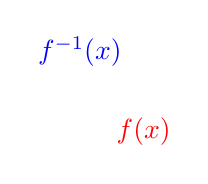
\begin{tikzpicture}[scale=1]
    \tkzInit[xmin=-2, xmax=2, ymin=-2,ymax=2]
        %\tkzDrawXY
        \tkzAxeXY[fill=black!5]
        
        \tkzFct[thick,red]{0.5*x}

        \tkzFct[thick,blue]{2*x}
        \tkzFct[gray]{x}

        \draw[red, above right] (2,1) node{$f(x)$};
        \draw[blue, above right] (1,2) node{$f^{-1}(x)$};
        %\tkzDefPointByFct[ref=A, with=a](-1)
        %\tkzDefPoint(0,4){A}
        %\tkzDefPoint(2,0){B}
        %\tkzPointShowCoord(A)
        %\tkzDrawPoint[fill=red, size=3](A)
        %\tkzDrawPoint[fill=red, size=3](B)
    \end{tikzpicture}
    \end{center}
\end{exem}

\begin{exem}
    Seja $f:\R_{+}\to\R_{+}$ dada por $y=f(x)=x^2$. Como é bijetora, sua função inversa é dada por
    \begin{align*}
        x =y^2 \ \  \Rightarrow \ \ y =\sqrt{x} \Rightarrow \ \ f^{-1}(x) =\sqrt{x}.
    \end{align*}

    Seu gráfico é dado por
    \begin{center}
    \begin{tikzpicture}[scale=1]
    \tkzInit[xmin=0, xmax=3, ymin=0,ymax=3]
        %\tkzDrawXY
        \tkzAxeXY[fill=black!5]
        
        \tkzFct[thick,red]{x**2}

        \tkzFct[thick,blue]{sqrt(x)}
        \tkzFct[gray]{x}

        \draw[red, above left] (1.5,2) node{$f(x)$};
        \draw[blue, below right] (2,1.5) node{$f^{-1}(x)$};
        %\tkzDefPointByFct[ref=A, with=a](-1)
        %\tkzDefPoint(0,4){A}
        %\tkzDefPoint(2,0){B}
        %\tkzPointShowCoord(A)
        %\tkzDrawPoint[fill=red, size=3](A)
        %\tkzDrawPoint[fill=red, size=3](B)
    \end{tikzpicture}
    \end{center}
\end{exem}
% \begin{exem}
%  A função $f: \R \rightarrow \R$ dada por $f(x)= x+2$ é injetora, e sobrejetora portanto, existe uma função $g: \R \rightarrow \R$ dada por $g(x)= x-2$, tal que:
% \begin{eqnarray}
% (f \circ g)(x)&=& (x-2) + 2= x-2+2= x \\
% \Rightarrow (f \circ g)(x)&=& Id(x)
% \end{eqnarray}
% e ainda,
% \begin{eqnarray}
% (g \circ f)(x)&=& (x+2) - 2= x+2-2= x \\
% \Rightarrow (g \circ f)(x)&=& Id(x) ,
% \end{eqnarray}
% logo $g= f^{-1}$ é a função inversa de $f$.

%  \begin{figure}[H]
%  \centering
%     \fbox{\includegraphics[width=8cm]{./cap_funcao/figs/funcao_composta}}
%     \caption{Composta das funções $f$ e $g$}
%   \end{figure}

% \end{exem}

\begin{secExercicios}

\begin{exer}
    Se $f(x)=5x+3$ e $h(x)=1-2x$, calcule $f(h(1))+h(f(1))$.
\end{exer}

\begin{exer}
    Dadas as funções $f(x)=x^2+2x$ e $g(x)=-3x+1$ com domínios reais, determine:
    \begin{enumerate}[a)]
    \begin{multicols}{3}
        \item $f(g(x))$
        \item $g(f(x))$
        \item $f(f(x))$
    \end{multicols}
    \end{enumerate}
\end{exer}

\begin{exer}
    Dadas $f(x)=2x+1$ e $f(g(x))=2x+9$, determine $g(x)$.
\end{exer}

\begin{exer}
    Sejam $f(x)=\sqrt{x-1}$ e $g(x)=2x^2-5x+3$. Determine o maior domínio das funções $f\circ g$ e $g\circ f$.
\end{exer}

\begin{exer}
    Sejam $f(x)=\dfrac{x+1}{x-2}$ e $g(x)=2x+3$. Determine o maior domínio das funções $f\circ g$ e $g\circ f$.
\end{exer}

\begin{exer}
    Para cada uma das funções a seguir, diga se é injetora, sobrejetora, bijetora ou nenhum dos casos.
    \begin{enumerate}[a)]
        \item $f:(-1,1)\to \R$, com $f(x)=x^3$.
        \item $f: \R^*\to\R^*$, com $f(x)=\frac{1}{x}$.
        \item $f:\R\to\R$, com
        $f(x)= \left\{
            \begin{matrix}
                x^2, & \mbox{se } x\geq 0\\
                x, & \mbox{se } x<0.
            \end{matrix}
            \right.$

        \item $f:\R\to\R$,
       $f(x)= \left\{
            \begin{matrix}
                x-1, & \mbox{ se } x\geq 1\\
                0, & \mbox{ se } -1< x< 1\\
                x+1, & \mbox{ se } x\leq -1.
            \end{matrix}
            \right.$
    \end{enumerate}
\end{exer}

\begin{exer}
    Determine a função inversa de cada uma das funções definidas de $\R$ em $\R$:
    \begin{enumerate}[a)]
        \begin{multicols}{2}
            \item $f(x)=3x+2$
            \item $f(x)=\frac{4x+1}{3}$
            \item $f(x)=x^3+2$
            \item $f(x)=(x-1)^2+2$
            \item $f(x)=\sqrt[3]{x+2}$
            \item $f(x)=\sqrt{1-x^2}$
        \end{multicols}
    \end{enumerate}
\end{exer}

\begin{exer}
    A função $f:\R\to\R$ dada por $f(x)=x^4+1$ admite inversa? Justifique sua resposta.
\end{exer}

\begin{exer}
    Considere a função $f:[a,+\infty)\to\R_+$ dada por $f(x)=x^2-2x+1$, onde $a$ é algum valor real constante.
    \begin{enumerate}[a)]
        \item Qual é o menor valor de $a$ de modo que $f$ seja injetora?
        \item Determine sua função inversa.
    \end{enumerate}
\end{exer}

\begin{exer}
    Considere a função real $f:A\to B$ dada pela expressão
    \begin{equation*}
        f(x)=\dfrac{x+2}{x+1}.
    \end{equation*}
    \begin{enumerate}[a)]
        \item Determine $A$ e $B$ de modo que $f$ seja inversível.
        \item Calcule $f^{-1}$.
        \item Esboce os gráficos de $f$ e $f^{-1}$.
    \end{enumerate}
\end{exer}
\end{secExercicios}

%\subsection*{Respostas}
%\shipoutAnswer


